\documentclass{article}
\bibliographystyle{ieeetr}
\usepackage{graphicx} 
\usepackage{svg}

\title{Echocardiography Guidance and Training with Mixed Reality}
\author{Edvart G. Bjerke}
\date{March 2025}

\begin{document}
\maketitle

\section{Introduction}
The aim of this thesis is to implement a guidance and training system in augmented reality. The system is targeted at trainees, students and other unskilled practitioners. The goal is to provide a tool that is helpful both in learning about how to perform echocardiographic examinations and in actual examinations.

A pre-trained deep neural network- based model will be used to generate guidance signals for the user, and these signals will be integrated into the augmented reality system.  
Additionally, virtual reference model placed in the virtual environment allows the user to explore cardiac structures and familiarize themselves with
standard views. 

The reference models are based on cardiac MRI data. 
Since the project is focused on echocardiography, it's essential that the reference model also includes ultrasound data.
This data should be spatially complete such that the user can view scan planes from arbitrary poses in a continuous manner.
To maintain coherence, all representations (raw MRI, solid model and ultrasound) are obtained from the same patient. This ensures that context is not lost when switching between representations.

Obtaining dense 4D ultrasound data that coheres with the MRI data from manual scanning is impractical. Instead,
echo data is simulated based on the solid model manually generated by contouring the 4D MRI data.

\section{Echocardiography}
Echocardiography examinations provide information about the patient's heart used to diagnose various 
cardiovascular disorders. Today, echocardiography is used extensively, as the procedure is low-cost and non-invasive \cite{Omerovic2023}.

In echocardiography, ultrasound signals are transmitted by a probe. The signal propagates through the medium of the patient and echoes are recorded
by the probe. These echoes are processed by a set of signal processing algorithms commonly referred to as "beamforming". The result of beamforming is a
greyscale image representing anatomical structures.


\section{Computer Graphics}
Computer graphics (CG) is the study of digitally generating images, videos, and other types of graphical content.
The type of visual content generated can broadly be categorized into photorealistic and non-photorealistic CG.
The applications of CG techniques are broad- including scientific visualizations, video games, special effects and other types of informative or artistic content.

Algorithms in computer graphics typically operate on objects of a three-dimensional (3D) \textit{scene}. The scene is a high-level description of the virtual environment used to synthesize the visual content.
The objects in the scene may represent things like solid bodies, cameras, light sources or arbitrary volumetric data.

\subsection{Rendering}
Rendering algorithms generate digital images, given a set of objects from the scene. These algorithms
are often physically-based, where \textit{photorealistic} techniques simulate real light phenomena to produce visually realistic results. 


\textit{Non-photorealistic} rendering techniques are used when photorealism is n    ot desired- whether for aesthetic purposes or when the objects represent something
invisible to the human eye. 

\subsection{The Graphics Pipeline}
The graphics pipeline is a high-level description of the sequence of processes used to 
generate an image from the scene description. The graphics pipeline is not rigidly defined,
and different architectures are used to render different tyepes of data or to achieve results of a particular aesthetic.

In real-time computer graphics, the graphics pipeline can generally be viewed as three parts- the application, geometry processing and rasterization \cite{RealTimeRendering}.

\begin{figure}[tbh]
    \centering
    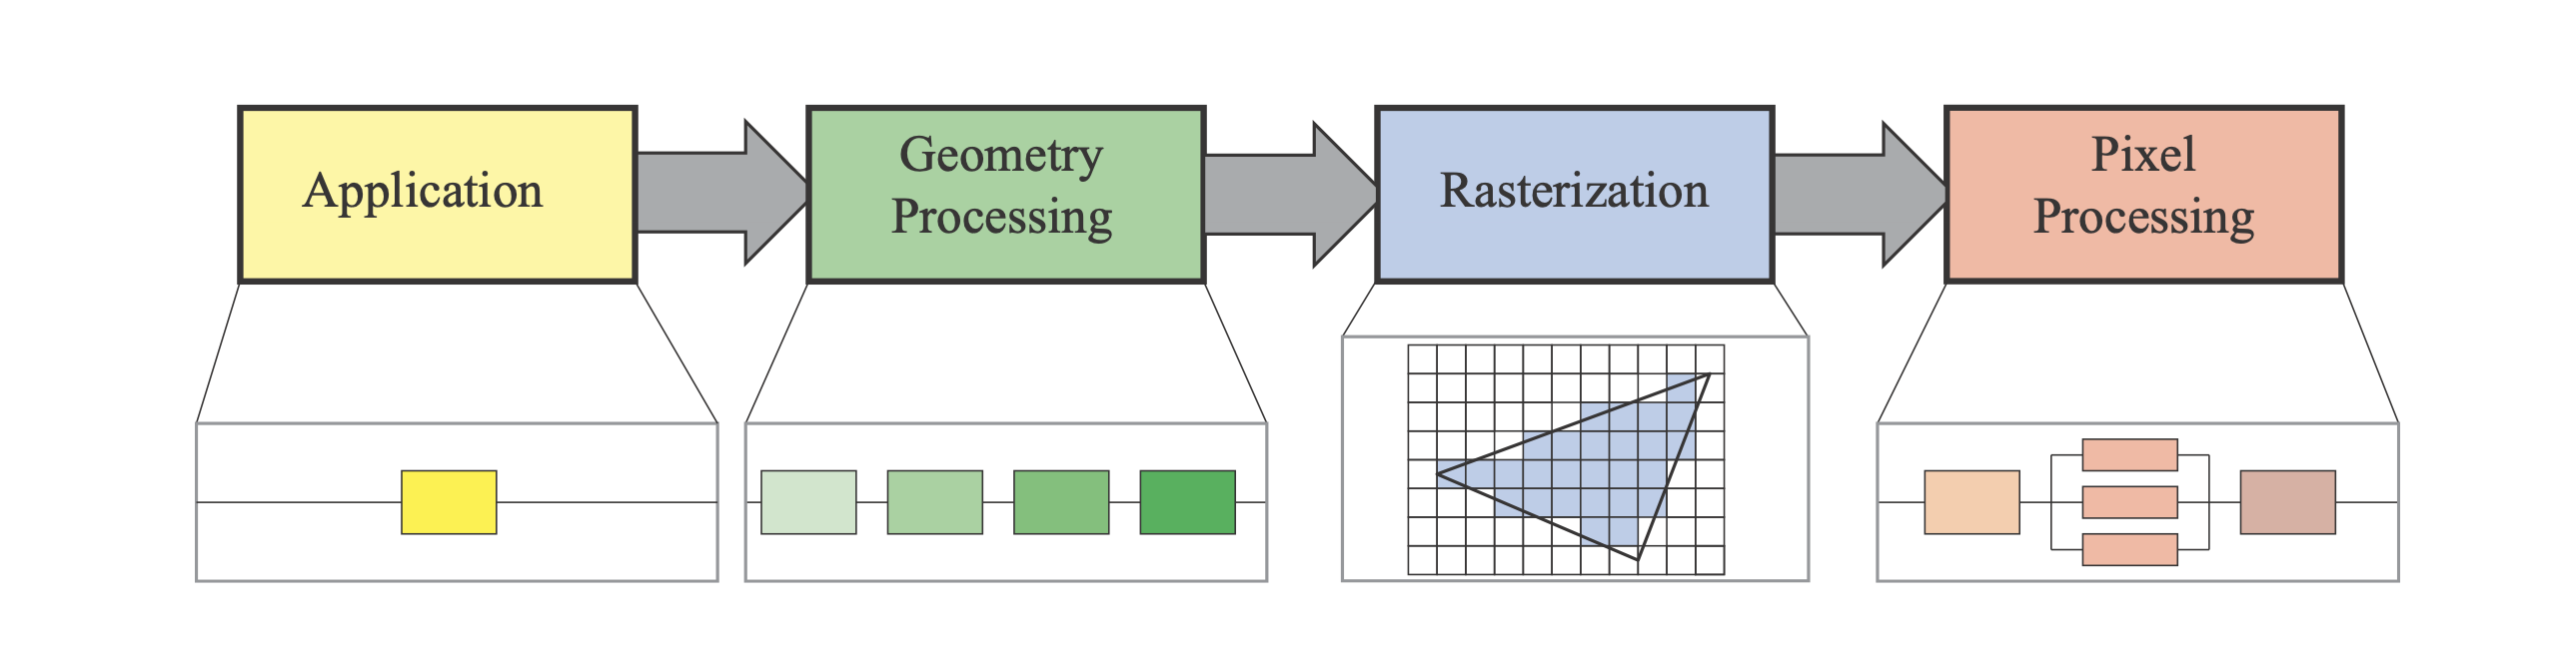
\includegraphics[width=1.0\textwidth]{images/graphics_pipeline.png}
    \caption{The graphics pipeline \cite{RealTimeRendering}}
    \label{fig:pipelineRealTimeRendering}
\end{figure}

The application part of the pipeline generally runs on the CPU, and is concerned with defining the structure of the scene, setting up rendering commands and other pre-processing procedures.
The application defines a set of geometry \textit{primitives} which are sent further down the pipeline. These primitives
are geometrical shapes like triangles and lines, defined by coordinates and indices defining the surface of the models to be processed and rendered by the GPU.
The data strutures representing these primitives are typically defined in a local coordinate system referred to as \textit{object space}, and may include additional information such as surface normals and texture coordinates. The data required
in this stage depends on the algorithms employed in the \textit{pixel processing} stage of the pipeline.

The geometry processing stage is executed on the GPU, where geometrical operations like morphing and subdividing (tesselation) may be performed.
An essential part of the geometry processing stage is the \textit{vertex shader}, which is a programmable procedure which processes each 3D vertex (position) of the given mesh.

In a typical rendering pipeline, the vertex shader transforms the vertex coordinates from \textit{object space} to \textit{screen space} through perspective projection, such that
objects are correctly rendered to the screen according to the \textit{pinhole camera model}.

\begin{figure}[tbh]
    \centering
    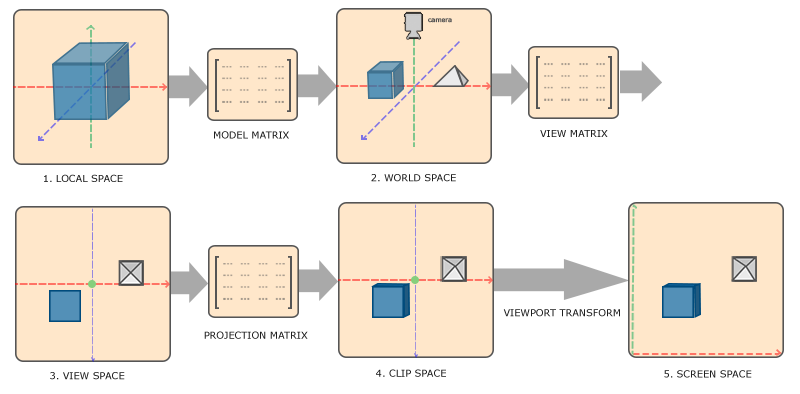
\includegraphics[width=1.0\textwidth]{images/coordinate_systems.png}
    \caption{Representation of geometry processing in a standard vertex shader using perspective projection\cite{learnopengl_figure}.}
    \label{fig:graphicsTransformations}
\end{figure}

The rasterization part of the pipeline uses the screen space coordinates computed by the vertex shader to
determine the set of pixels covered by the projection of the primitive. 

Finally, the colors of the rasterized pixels are determined in the pixel processing stage.
The GPU program defining the algorithm used for shading pixels is referred to as the \textit{fragment shader}.
The fragment shader is executed in parallell, for each rasterized pixel. With modern GPUs and graphics frameworks, fragment shaders are highly programmable, and different shaders may be used to render different objects.

\subsection{Volume Rendering}
The traditional raster-based rendering technique is not well-suited for rendering phenomena that are volumetric in nature.
Special rendering techniques have been developed to render physically occuring phenomena like smoke, clouds or fog. These techniques
may also be used to visualize three-dimensional scientific data, like that captured by fluid simulation or medical imaging.

\begin{figure}[tbh]
    \centering
    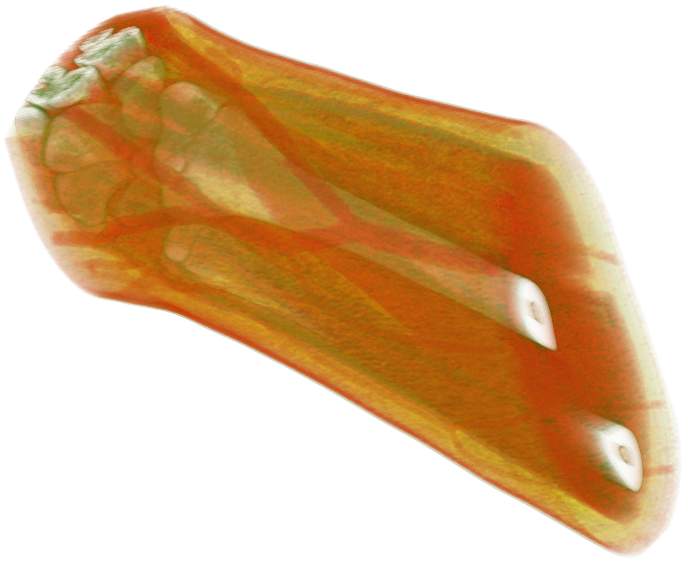
\includegraphics[width=1.0\textwidth]{images/VolumeRendering.png.png}
    \caption{Volume rendering of a CT scan of a forearm}
    \label{fig:graphicsTransformations}
\end{figure}



\bibliography{references}
\end{document}
